\chapter{Something about strained hBN}
\chaptertoc{}

\section{oui}

\begin{itemize}
	\item experimental motivations
	\item why we build the orthorombic cell 
	\item relaxation of the structures (I didn't mention structure relaxtion with DFT anywhere)
	\item convert orthorombic to pseudo-hexagonal (this could be an appendix)
	\item alot of computational details
	\item electronic band structure 
	\item exciton-phonon coupling from finite differences
	\item vRS relation in this case 
\end{itemize}
%
%
ETSF webinar of Fulvio
indirect bandgap only; we can write the response function with derivatives of the response function because we consider only phonon-assisted transitions; need supercells
converge the displacement so that it is the smallest possible
PLE (propto absorption) or absorption and PL are not symmetric, as expected for direct gaps
the minimum exciton at T is the degenerate dark state at Gamma which splits
for absorption, the bright exciton overlaps with the phonon replicas and it is so bright that we don't see them 
%
%
Theory of phonon-assisted optics : it exists. For instance, Williams-Lax theory that treats lattice-dependent band features and phonon-assisted transitions 
There is also Hallen-Bardeen-Blatt and Heine-Cardona but I don't know too much about them.
Besides, some models of exciton-phonon coupling exists also, some specifically for luminescence, but they are computationally expensive for real materials.
==> there is a need for exciton-phonon coupling and phonon-assisted optics from first principles. In the next two chapters, two different approaches are presented. The first one consists in calculating the response function correction due to exciton-phonon coupling from finite differences, by displacing atoms in supercells. The second one is a more general approach based on \acrshort{MBPT}, in which a dynamical correction induced by electron-phonon coupling is added as a perturbation to the Bethe-Salpeter kernel. Thanks to this \textit{ab initio} framework, the scattering of every exciton with every phonon mode can be computed, over the whole Brillouin Zone. These calculations are done in the unit cell.
Both approaches allow to compute the exciton-phonon coupling. Then, the absorption can be obtained after post-processing of a standard \acrshort{BSE} calculation. To obtain the luminescence spectra, we use the van Roosbroeck -- Shockley relation for both cases.

\subsection{Experimental motivations}
From Léonard Schué's thesis, (suspended nanosheet of hBN), they conclude that there is probably a residual uniaxial strain at the center of the suspended sheet. They use cathodoluminescence, where the electron beam penetrates in the bulk of the crystal

In this experiment, the group of Julien Barjon, specifically Léonard Schué, they suspended a nanosheet of hexagonal Boron Nitride on a over a trench carved out from an SiO$_2$ substrate. The nanosheet is about 100 nm thick and curves under the effect of gravity, as illustrated in Fig. \ref{fig:exp_strain}(a), and was imaged by \acrfull{AFM} (Fig. \ref{fig:exp_strain}(b)).
\begin{figure}[h!tbp]
	\vspace{0.5cm}
	\setcapindent{2em}
	\centering
	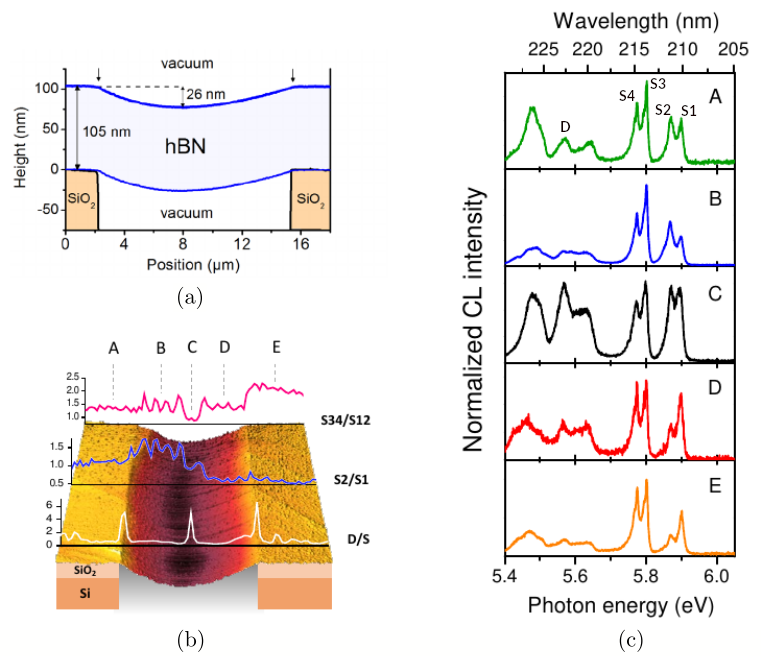
\includegraphics[width=0.8\textwidth]{exp_strain.png}
	\caption{(a) Sketch of the deposited hBN nanosheet on the trench. (b) AFM profile and relative intensity ratios of different emission peaks with respect to spatial region. (c) Cathodoluminescence intensity measured on different regions of the sample.}
	\label{fig:exp_strain}
\end{figure}
When measuring the cathodoluminescence spectra at different positions on the sample, one can see that the intensity ratios between different peaks are varying. Their interpretation is that the deformation of the sample induces uniaxial (compressive) strain, perpendicular to the trench. This strain could have an effect on the recombination process of excitons, leading to a change in the luminescence intensity.
%
%
\subsection{Structure and phonons}
We try to simulate the experimental strained structure by , focusing mainly on compressive strain because the electron beam penetrates on the upper part of the sample where the strain is compressive.